
\section{Monte Carlo Integration}
\label{sec: monte carlo integrals}

Equations~\ref{eq: single event estimator} and~\ref{eq: selection effects estimator} are examples of Monte Carlo integrals. In this section, we discuss the basic theory of Monte Carlo integration, the uncertainty in estimators, and biased and unbiased estimation.

Monte Carlo integration is a technique for estimating the value of an integral stochastically. Take many random draws from the domain of integration using a known probability density which is easy to sample, then reweight to the integrand function. Specifically, given an integral 
\beq
I = \int f(\theta) \dd\theta,
\eeq
and $M$ independent draws from a distribution $\theta_i \sim p(\theta)$, the Monte Carlo estimate of the integral is (see chapter 29 of \citet{MacKay2003})
\beq
\hat{I} = \frac{1}{M}\sum_{i=1}^M \frac{f(\theta_i)}{p(\theta_i)}.
\eeq
Monte Carlo integration is a general technique for estimating nonelementary or high dimensional integrals, because the uncertainty in the estimate is not explicitly dependent on the dimension of the domain of the integral. 

We can compute the expectation of the estimator
\beq
\langle\hat{I}\rangle = \int \left(\frac{1}{M}\sum_{i=1}^M \frac{f(\theta_i)}{p(\theta_i)}\right) p(\theta_1) \dd\theta_1 p(\theta_2) \dd\theta_2 ... p(\theta_M) \dd\theta_M  = \frac{1}{M}\sum_{i=1}^M \int \left(\frac{f(\theta_i)}{p(\theta_i)}\right)p(\theta_1)\dd\theta_1 p(\theta_2) \dd\theta_2 ... p(\theta_M) \dd\theta_M
\eeq
using the fact that integration is linear. Notice that for the $i^{\rm th}$ term in the sum, the integrand is independent of all but one of the integration variables $\theta_i$, and all others integrate away to 1. Therefore, 
\beq
\langle\hat{I}\rangle = \frac{1}{M}\sum_{i=1}^M \int \left(\frac{f(\theta_i)}{p(\theta_i)}\right)p(\theta_i)\dd\theta_i = \frac{1}{M}\sum_{i=1}^M \int f(\theta_i) \dd\theta_i = \int f(\theta)\dd\theta = I.
\label{eq: expectation of Monte Carlo integral}
\eeq
Because the expectation of the Monte Carlo integral is correct ($\expect{\hat{I}} = I$), we call the Monte Carlo estimator $\hat{I}$ an \textit{unbiased} estimator for $I$. We should note, however, that the simplification in Eq.~\ref{eq: expectation of Monte Carlo integral} only works if $p(\theta) > 0$ wherever $f(\theta) \neq 0$. Otherwise, the estimator is in general \textit{biased}. You cannot re-weight a distribution outside its domain.

Using a similar approach, we can compute the variance of the estimator as 
\beq
\variance{\hat{I}} = \langle(\hat{I} - \expect{I})^2\rangle = \frac{1}{M}\left(\int \frac{f(\theta)^2}{p(\theta)}\dd\theta - I^2\right),
\label{eq: variance of Monte Carlo integral}
\eeq
which is just a constant value suppressed by a factor of $M^{-1}$. This gives the Monte Carlo integral the attractive property that the uncertainty can be decreased as much as we like, simply by drawing more samples. How \textit{much} we must increase the number of samples, however, depends sensitively on how similar $p(\theta)$ is to $f(\theta)$: the integral in Eq.~\ref{eq: variance of Monte Carlo integral} can be extremely large or even infinite for poorly chosen $p(\theta)$. Indeed, there is a similar issue as Eq.~\ref{eq: expectation of Monte Carlo integral}. If there is a finite-measure subset of the domain where $f(\theta) \neq 0$ but $p(\theta) = 0$, then the variance diverges \textit{for all} $M$. Even if the domain where $f(\theta) \neq 0$ also has $p(\theta) \neq 0$, if $p(\theta)$ becomes too small faster than $f(\theta)$, the variance may still diverge.

% We can use variational calculus to show that the optimal draw probability distribution is just the normalized absolute value of $f(\theta)$
% \beq
% p_{\rm opt}(\theta) = \frac{|f(\theta)|}{\int |f(\theta')|\dd\theta'}
% \eeq
% This is a double edged sword, however. Monte Carlo integration converges frustratingly slow compared to other integration estimation techniques, and we should only use it when all other options are worse \fixme{cite that integration review book}

% the variance is zero for the optimal draw distribution iff f(\theta) >= 0 almost everywhere. If f(theta) >= 0, then the variance is zero under the optimal draw distribution, because obviously: the normalization already contains the intgral we want to calculate.

Just as we are able to estimate $\hat{I} \approx I$ with Monte Carlo integration, we can estimate $\mathbb{V}[\hat{I}]$ with
\beq
\hat{\sigma}^2_{I} = \frac{1}{M} \left( \frac{1}{M-1} \sum\limits_i^M \left(\frac{f(\theta_i)}{p(\theta_i)} - \hat{I} \right)^2 \right) = \frac{1}{M-1}\left(\frac{1}{M}\sum_{i=1}^M\frac{f(\theta_i)^2}{p(\theta_i)^2} - \hat{I}^2\right),
\label{eq: variance estimator}
\eeq
which is also an unbiased estimator: $\expect{\hat{\sigma}^2_I} = \mathbb{V}[\hat{I}]$ (this fact can be shown by exactly the same procedure as Eq.~\ref{eq: expectation of Monte Carlo integral}), provided the variance exists. Note the denominator $M-1$ rather than $M$---known as Bessel's correction---is required for the estimator to be unbiased \citep{kendall1977advanced}.
Since Eqs.~\ref{eq: single event estimator} and~\ref{eq: selection effects estimator} are Monte Carlo integrals, they are unbiased estimators for the corresponding integrals: $\langle\hat{p}(d_i|\Lambda)\rangle = p(d_i|\Lambda)$ and $\langle\hat{\xi}(\Lambda)\rangle = \xi(\Lambda)$.\footnote{To be precise, $\hat{\xi}(\Lambda)$ should be thought of as a Monte Carlo integral over the space of all data $d$ and sources $\theta$ as opposed to a Monte Carlo integral over only the space of sources $\theta$. Using the expression in the center of Eq.~\ref{eq: selection effects estimator}, the expectation can be taken directly over the sources $d_j, \theta_j$, without accounting for the data-dependent $N_{\rm found}$.}


However, while the variance in each Monte Carlo integral is important, a more appropriate quantity to track is the total variance in the log-likelihood estimator in Eq.~\ref{eq: estimated hierarchical likelihood}. The variance in each Monte Carlo ingredient propagates to the total log-likelihood variance as
\beq
\hat{\sigma}^2_{\ln\mathcal{L}}(\Lambda) = \left(\sum_{i=1}^{\Nobs}\frac{\hat{\sigma}^2_{p_i}}{\hat{p}(d_i|\Lambda)^2}\right) + \frac{\Nobs^2\hat{\sigma}^2_{\xi}}{\hat{\xi}(\Lambda)^2},
\label{eq: likelihood variance estimator}
\eeq
where $\hat{\sigma}^2_{p_i}$ is the variance calculated from Eq.~\ref{eq: variance estimator} for $\hat{p}(d_i|\Lambda)$ and $\hat{\sigma}^2_{\xi}$ is the variance for $\hat{\xi}(\Lambda)$.
\citet{Talbot:2023pex} conjecture that thresholding on this variance estimator ensures a safe hyperposterior. By using a generalization of Eq.~\ref{eq: likelihood variance estimator}---the covariance in the log-likelihood at two hyperparameters $\Lambda$ and $\Lambda'$, first introduced by \citet{Essick:2022ojx}---we show in Sec.~\ref{sec: robustness measures} that the log-likelihood variance threshold indeed ensures a safe hyperposterior.

\subsection{Nonlinear functions of a Monte Carlo integral}
\label{subsec: monte carlo bias}

In the hierarchical likelihood for a population inference (Eq.~\ref{eq: rate marginalized likelihood}), we must multiply by a selection efficiency integral, raised to the negative power of the number of events in the catalog $\Nobs$. That is, we run the estimator $\hat{\xi}(\Lambda)$ through the function $g(x) = x^{-\Nobs}$. We may write the expectation of this nonlinear function of the Monte Carlo integral
\beq
\expect{g(\hat{I})} = \expectlarge{\hat{I}^{-\Nobs}} = \int \left(\frac{1}{M}\sum_{i=1}^M \frac{f(\theta_i)}{p(\theta_i)}\right)^{-\Nobs} p(\theta_1) \dd\theta_1 p(\theta_2) \dd\theta_2 ... p(\theta_M) \dd\theta_M \neq I^{-\Nobs}
\eeq
which cannot be simplified using the techniques from before. In fact, this is generically a \textit{biased} estimator for $I^{-\Nobs}$, and since $g(x) = x^{-\Nobs}$ is a convex function for $x > 0$, then, by Jensen's inequality, the estimator is biased \textit{too large}: $\expect{\hat{I}^{-\Nobs}} > I^{-\Nobs}$ \citep{kendall1977advanced, MacKay2003}. 

We can approximate the bias by a Taylor expansion to leading order. Expanding each weight $f(\theta_i) / p(\theta_i)$ around the expectation of that weight, $\expect{f(\theta_i) / p(\theta_i)} = I$, 
\beq
\expect{g(\hat{I})} \approx \int \left[g(I) + \frac{g'(I)}{M} \sum_{i=1}^M \left(\frac{f(\theta_i)}{p(\theta_i)} - I\right)  + \frac{g''(I)}{2M^2}\sum_{i=1}^M \left(\frac{f(\theta_i)}{p(\theta_i)} - I\right)^2 + \mathcal{O}\left(\frac{1}{M^2}\right)\right] p(\theta_1) \dd\theta_1 p(\theta_2) \dd\theta_2 ... p(\theta_M) \dd\theta_M,
\eeq
where $g'(I)$ and $g''(I)$ are the first and second derivatives of $g$, evaluated at $I$. Using the same techniques as in Eq.~\ref{eq: expectation of Monte Carlo integral} and Eq.~\ref{eq: variance of Monte Carlo integral}, we can simplify to
\beq
\expect{g(\hat{I})} \approx g(I) + \frac{g''(I)}{2}\variance{\hat{I}} + \mathcal{O}\left(\frac{1}{M^2}\right) = I^{-\Nobs}\left[1 + \frac{\Nobs(\Nobs + 1)}{2}\frac{\variance{\hat{I}}}{I^2} + \mathcal{O}\left(\frac{1}{M^2}\right)\right].
\label{eq: bias for mean raised to power}
\eeq

The approach of Eq.~\ref{eq: bias for mean raised to power} does not assume anything about the distribution for $\hat{I}$ beyond that the mean and variance exist. However, we can make a more reasonable assumption about the distribution of $\hat{I}$, namely, that it is distributed as a normal distribution by the central limit theorem. If we assume $M$ is sufficiently large, we can assume that the normal distribution is narrow, and thus can also be approximated as a narrow log-normal distribution. It is easy to raise a log-normal distribution to an arbitrary power, and under this assumption one obtains that (also shown in \citet{Essick:2022ojx})\footnote{Another advantage of a log-normal distribution is that it only has support for positive values, and we know the estimator must be positive.}
\beq
\expect{\hat{I}^{-\Nobs}} \approx I^{-\Nobs}\exp\left(\frac{\Nobs(\Nobs + 1)}{2}\frac{\variance{\hat{I}}}{I^2}\right).
\label{eq: bias for mean raised to power assuming lognormal}
\eeq
For an illustrative example, consider the simple case where we want to estimate the integral of an exponential function raised to the $\Nobs=-100$ power
\beq
I_{\rm expo}^{-100} = \left(\int_0^\infty e^{-x} \dd x\right)^{-100} = 1.
\eeq
Pretending that we don't already know the analytic value, let's use a Monte Carlo estimator with draws from a \textit{broader} exponential $x_i \sim p(x) = \frac{1}{2}e^{-x/2}$,
\beq
\hat{I}_{\rm expo}^{-100} = \left(\frac{1}{M}\sum_{i=1}^M \frac{2e^{-x_i}}{e^{-x_i/2}}\right)^{-100} = \left(\frac{1}{M}\sum_{i=1}^M 2e^{-x_i/2}\right)^{-100}.
\label{eq: exponential reweighting scheme}
\eeq
We can compute the variance in closed form, which gives us the expectation
\beq
\variance{\hat{I}_{\rm expo}} = \frac{1}{3M} \implies \expect{\hat{I}_{\rm expo}^{-100}} = \begin{dcases}
1 + \dfrac{5050}{3M} + \mathcal{O}\left(\dfrac{1}{M^2}\right) & \text{to leading order} \\
\exp\left(\dfrac{5050}{3M}\right) & \text{assuming log-normal}
\end{dcases}
\label{eq: expectation of exponential biased estimator}
\eeq
To verify these approximations, we show the histograms of many random realizations using different fixed values of $M$ in Fig.~\ref{fig: exponential powers histograms} and a comparison of the empirical expectation with the theoretical expectation of this biased estimator (Eq.~\ref{eq: expectation of exponential biased estimator}) as a function of $M$. 

\begin{figure}
    \centering
    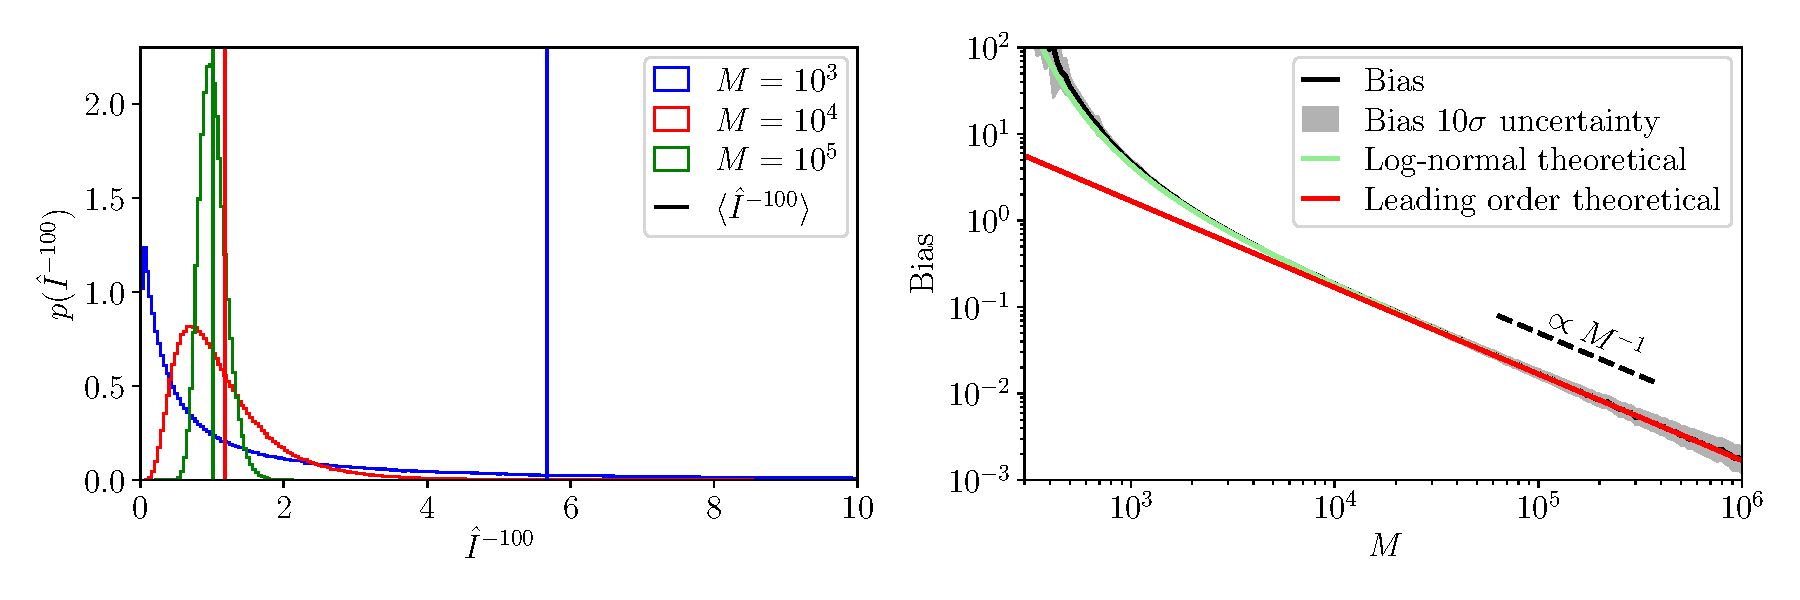
\includegraphics[width=\linewidth]{plots/exponetial_powers_hist_linscale.pdf}
    \caption{
    \textit{Left}: Histograms of $10^6$ draws of a $\hat{I}^{-100}$ estimated from reweighting a sample of $M$ values from a broader exponential distribution, for various values of $M$. The solid vertical lines show the mean of these draws, $\expect{\hat{I}^{-100}}$. The mean becomes severely biased for small $M$, as the distribution of $\hat{I}^{-100}$ becomes strongly skewed. 
    \textit{Right}: The bias $\expect{\hat{I}^{-100}} - I^{-100}$ as a function of $M$. In black is the empirical bias computed from an average of $10^6$ estimates with sample size $M$, with the $10\sigma$ (so the envelope is visible) shaded uncertainty envelope. The uncertainty is due to averaging with finite number statistics ($10^6$). In green is the theoretical bias assuming the $\hat{I}$ is distributed according to a log-normal, which closely matches the empirically calculated bias, and in red is the leading order theoretical bias, which does not assume an underlying distribution for $\hat{I}$ but deviates at small values of $M$ (see Eq.~\ref{eq: expectation of exponential biased estimator}).
    }
    \label{fig: exponential powers histograms}
\end{figure}

\subsection{Correction Factor}

We can correct for the bias due to the nonlinearity using a correction factor, which we derive in general in Appendix~\ref{app: correction in general}, under the restrictions that the improved estimator should remain positive everywhere, and remove the leading order bias. For the function $g(x) = x^{-\Nobs}$, the corrected estimator for $I^{-\Nobs}$ is
\beq
\hat{I}_{\rm corr}^{-\Nobs} \equiv \hat{I}^{-\Nobs}\exp(-\frac{\Nobs(\Nobs+1)}{2}\frac{\hat{\sigma}^2_{I}}{\hat{I}^2}).
\label{eq: corrected integral power estimator}
\eeq

Having removed the leading order bias at $\mathcal{O}(M^{-1})$, the remaining bias occurs at $\mathcal{O}(M^{-2})$. We show the analogous figure to Fig.~\ref{fig: exponential powers histograms} in Fig.~\ref{fig: corrected exponential powers histograms} and verify the remaining bias scales as expected. 
\begin{figure}
    \centering
    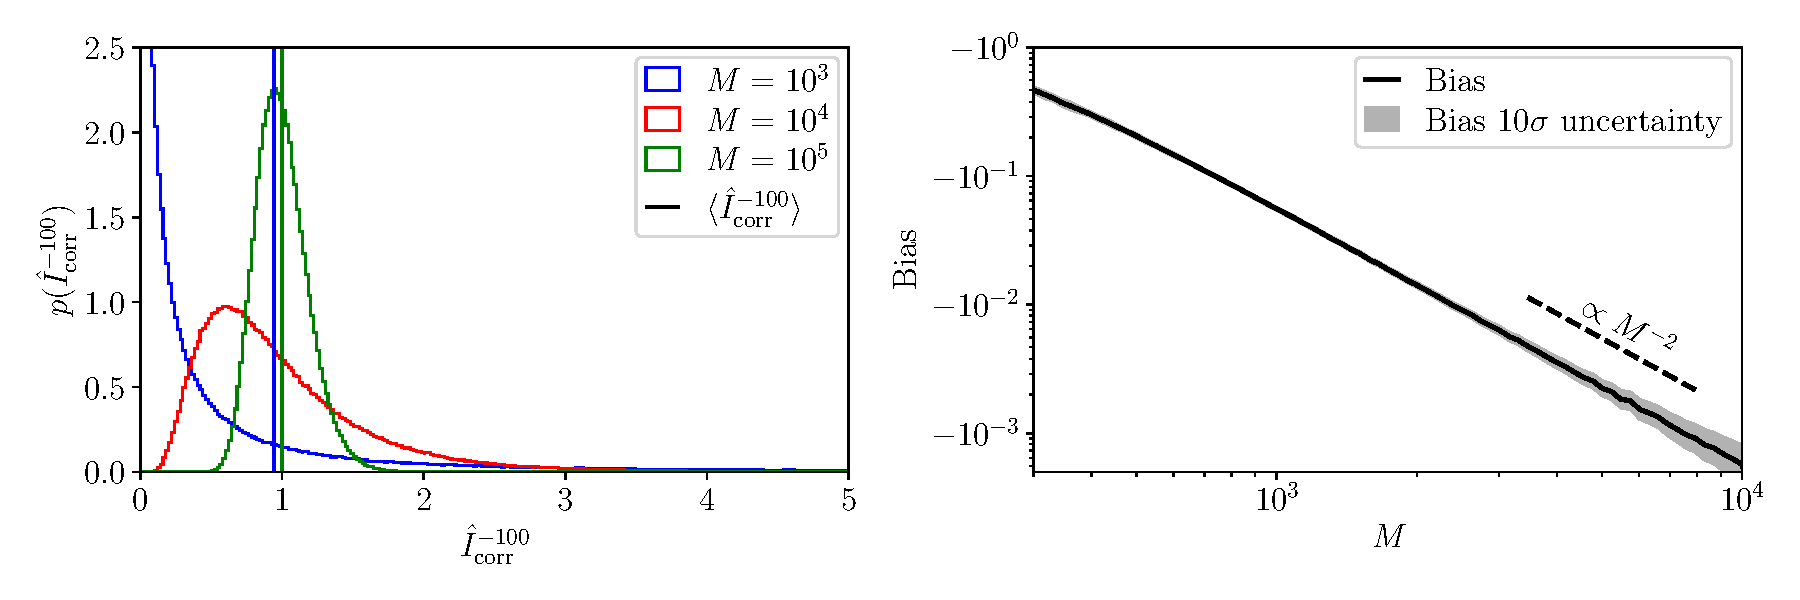
\includegraphics[width=\linewidth]{plots/exponetial_powers_corrected_hist_linscale.pdf}
    \caption{
    Analogous to Fig.~\ref{fig: exponential powers histograms} except using the corrected estimator $\hat{I}_{\rm corr}$. Note the bias is now negative and the reduced axes relative to Fig.~\ref{fig: exponential powers histograms}. We show the bias now scales as $\mathcal{O}(M^{-2})$ as expected.
    }
    \label{fig: corrected exponential powers histograms}
\end{figure}

\section{Bias in population inference}
\label{sec: bias in population inference}

%Having gone through the essentials of Monte Carlo integration and estimator theory, we are now ready to understand the source of bias in the likelihood and posterior estimators in \ac{GW} hierarchical inference.

\subsection{Likelihood bias and correction}

We saw in Section~\ref{subsec: monte carlo bias} that running an \textit{unbiased} Monte Carlo estimator through a nonlinear function produces a biased estimator. In \ac{GW} population analyses, the likelihood is estimated by raising the selection effects estimator to the $-\Nobs$ power: $\hat{\xi}(\Lambda)^{-\Nobs}$.
Without any correction, this means the likelihood estimator is biased as in Eqs.~\ref{eq: bias for mean raised to power} and \ref{eq: bias for mean raised to power assuming lognormal}. 

For an unbiased likelihood estimator, we need to include the following modifying term.\footnote{Note the similarity but opposite sign to the modifying term proposed \citet{Farr:2019rap}. Both approaches compute a bias term $\sim \exp(\Nobs^2/2\Neff)$, though \citet{Farr:2019rap} suggests including this term explicitly as a marginalization over the uncertainty. That is, the correction in \citet{Farr:2019rap} is analogous to the bias term in Eq.~\ref{eq: bias for mean raised to power assuming lognormal}. We suggest that the expectation of the likelihood should be unbiased, and so we \textit{undo} this term, hence it obtains a minus sign in Eq.~\ref{eq: unbiased likelihood estimator}.}
\beq
\hat{\mathcal{L}}_{\rm corr}(\{d_i\} | \Lambda) \equiv \hat{\xi}(\Lambda)^{-\Nobs}\exp\left(-\frac{1}{2}\frac{\Nobs(\Nobs+1)\hat{\sigma}_\xi^2(\Lambda)}{\hat{\xi}(\Lambda)^2}\right)\prod_{i=1}^{\Nobs}\hat{p}(d_i|\Lambda)
\label{eq: unbiased likelihood estimator}
\eeq
where $\hat{\sigma}^2_{\xi}$ is the estimated variance in the Monte Carlo integral for $\hat{\xi}$
\beq
\hat{\sigma}^2_\xi = \frac{1}{\Ninj-1}\left(\frac{1}{\Ninj}\sum_{j=1}^{\Ninj}\frac{p(\theta_j|\Lambda)^2}{p(\theta_j|{\rm draw})^2} - \hat{\xi}(\Lambda)^2\right).
\eeq
With the inclusion of the modifying term, the bias in the likelihood estimator is removed to leading order (that is, it is now at order $\Ninj^{-2}$ rather than $\Ninj^{-1}$). It does not reduce the precision of the estimator meaningfully, and so represent a simple improvement to the likelihood estimator. For the mathematical details on this modifying term, see the Appendices \ref{app: bias in general} and \ref{app: correction in general}.

Now since the estimators $\hat{\xi}(\Lambda)$ and $\hat{p}(d_i|\Lambda)$ are all uncorrelated---the Monte Carlo samples are from unrelated distributions---the expectation over Monte Carlo samples of the likelihood estimator in Eq.~\ref{eq: unbiased likelihood estimator} factors and is now unbiased to $\mathcal{O}(\Ninj^{-2})$
\beq
\expectlarge{\hat{\mathcal{L}}_{\rm corr}(\{d_i\} | \Lambda)} = \expectlarge{\hat{\xi}(\Lambda)^{-\Nobs}\exp\left(-\frac{1}{2}\frac{\Nobs(\Nobs+1)\hat{\sigma}_\xi^2(\Lambda)}{\hat{\xi}(\Lambda)^2}\right)}\prod_{i=1}^{\Nobs}\expect{\hat{p}(d_i|\Lambda)} = \mathcal{L}(\{d_i\}|\Lambda)[1 + \mathcal{O}(\Ninj^{-2})].
\eeq

\subsection{Posterior bias}

However, the issue with the bias extends beyond the likelihood. Even if the likelihood estimator is unbiased, the \textit{posterior} can be biased. This is for a similar reason as the bias in the likelihood: the posterior is a nonlinear function of the likelihood, and so marginalizing the posterior over the uncertainty in the likelihood will leave some residual bias. Mathematically, this is due to the nonlinearity in the normalization and covariance in the likelihood estimator between multiple locations in parameter space $\Lambda, \Lambda'$. Denoting $\mathcal{L}(\{d_i\}|\Lambda) = \mathcal{L}(\Lambda)$ and the scatter $\hat{\mathcal{L}}(\Lambda)/\mathcal{L}(\Lambda) -1 \equiv \hat{\delta}(\Lambda)$,
\begin{align}
\expect{\hat{p}(\Lambda|\{d_i\})} 
&= \expectlarge{\frac{\pi(\Lambda)\mathcal{L}(\Lambda)[1 + \hat{\delta}(\Lambda)]}{\int \dd\Lambda' \pi(\Lambda')\mathcal{L}(\Lambda')[1 + \hat{\delta}(\Lambda')]}} \label{eq: bias in posterior heuristic} \\
&\approx p(\Lambda)\left(1 + \expect{\hat{\delta}(\Lambda)} - \int \dd\Lambda' p(\Lambda')\expect{\hat{\delta}(\Lambda')} - \int \dd\Lambda' p(\Lambda')\expect{\hat{\delta}(\Lambda)\hat{\delta}(\Lambda')} + \int \dd\Lambda'\dd\Lambda''p(\Lambda')p(\Lambda'')\expect{\hat{\delta}(\Lambda')\hat{\delta}(\Lambda'')}\right) \nonumber
\end{align}
where we have defined $p(\Lambda) = \pi(\Lambda)\mathcal{L}(\Lambda) / \int \dd\Lambda' \pi(\Lambda')\mathcal{L}(\Lambda')$ as the true posterior, and we have used the binomial expansion to second order for the denominator. 
$\expect{\hat{\delta}(\Lambda)}$ is proportional to the bias in the likelihood, and is zero for an unbiased likelihood (or $\mathcal{O}(\Ninj^{-2})$ for the corrected likelihood in Eq.~\ref{eq: unbiased likelihood estimator}). Notice there are additional biasing terms in the posterior estimator, due to $\expect{\hat{\delta}(\Lambda)\hat{\delta}(\Lambda')}$ terms or two-point \textit{covariance} terms between different locations in parameter space. 

It may seem surprising that we should worry about nonlinearity in a normalization term that only appears implicitly in most applications. We discuss this in Appendix~\ref{app: normalization discussion}.

We derive the general bias to leading order in the Appendix~\ref{app: bias in general}. For the \ac{GW} population inference problem approximated with Monte Carlo integration (Eq.~\ref{eq: estimated hierarchical likelihood}), the bias $b$ is such that
\beq
\expect{\hat{p}(\Lambda | \{d_i\})} = p(\Lambda | \{d_i\})\left(1 +b(\Lambda) - \int b(\Lambda')\dd\Lambda' \right)
\eeq
where $b(\Lambda)$ varies across parameter space and the second term simply ensures the posterior remains normalized. To leading order, 
\beq
b(\Lambda) = \frac{1}{2}\frac{\Nobs(\Nobs+1)\mathbb{V}[\hat{\xi}(\Lambda)]}{\xi(\Lambda)^2} - \int C_{\ln\mathcal{L}}(\Lambda, \Lambda')p(\Lambda'|\{d_i\})\dd\Lambda'.
\label{eq: posterior bias}
\eeq
The first term is the bias from the nonlinearity at which the selection effects estimator enters the likelihood; $\mathbb{V}[\hat{\xi}(\Lambda)]$ is the variance in the estimator $\hat{\xi}(\Lambda)$. As shown in detail in Appendix~\ref{app: bias in general}, the second term is the \textit{posterior} bias where $C_{\ln\mathcal{L}}(\Lambda, \Lambda')$ is the covariance in the log-likelihood estimator between points $\Lambda$ and $\Lambda'$, and for the \ac{GW} population inference problem, may be estimated with
\beq
\hat{C}_{\ln\mathcal{L}}(\Lambda, \Lambda') = \sum_{i=1}^{\Nobs}\frac{\hat{C}_{p_i}(\Lambda, \Lambda')}{\hat{p}(d_i|\Lambda)\hat{p}(d_i|\Lambda')}
+ \frac{\Nobs^2\hat{C}_{\xi}(\Lambda, \Lambda')}{\hat{\xi}(\Lambda)\hat{\xi}(\Lambda')}
\label{eq: population covariance with selection}    
\eeq
where 
\beq
\hat{C}_{p_i}(\Lambda, \Lambda') = \frac{1}{\NPE - 1}\left(\left[\frac{1}{\NPE}\sum_{j=1}^{\NPE}\frac{p(\theta_{ij}|\Lambda)}{\pi(\theta_{ij}|{\rm PE})}\frac{p(\theta_{ij}|\Lambda')}{\pi(\theta_{ij}|{\rm PE})}\right] - \hat{p}(d_i|\Lambda)\hat{p}(d_i|\Lambda')\right)
\label{eq: single event covariance estimator}
\eeq
is the covariance between the estimators $\hat{p}(d_i|\Lambda)$ and $\hat{p}(d_i|\Lambda')$ and
\beq
\hat{C}_{\xi}(\Lambda, \Lambda') = \frac{1}{\Ninj - 1}\left(\left[\frac{1}{\Ninj}\sum_{j=1}^{\Nfound}\frac{p(\theta_j|\Lambda)}{p(\theta_j|{\rm draw})}\frac{p(\theta_j|\Lambda')}{p(\theta_j|{\rm draw})}\right] - \hat{\xi}(\Lambda)\hat{\xi}(\Lambda')\right)
\label{eq: selection covariance estimator}
\eeq
is the covariance between the selection efficiency estimators $\hat{\xi}(\Lambda)$ and $\hat{\xi}(\Lambda')$.
These covariances come from the fact that each estimator is using the \textit{same} sets of samples to reweight across $\Lambda$ parameter space (also see \citet{Essick:2022ojx} and \citet{Talbot:2023pex}).

We illustrate the intuition behind the posterior bias in Fig.~\ref{fig: schematic of posterior bias}. Suppose the true likelihood is a standard normal, and we have an unbiased likelihood estimator scattered by a zero-mean log-Gaussian process. Each draw from the scattering process represents a likelihood estimator $\hat{\mathcal{L}}$. We show several draws of the likelihood estimator in the left-hand panel of Fig.~\ref{fig: schematic of posterior bias}. Notice, due to the form of the log-Gaussian process, the uncertainty is small towards the negative end of the parameter space, and grows larger towards the positive end. We also show the true likelihood ($\mathcal{L}$, green) and the average of the likelihood estimators ($\langle\hat{\mathcal{L}}\rangle$, red) to show the likelihood estimator is unbiased, as designed.

\begin{figure}
    \centering
    
\includegraphics[width=0.8\linewidth]{plots/continuous_likelihood_bias_schematic.pdf}
    \caption{A schematic for how an unbiased likelihood estimator leads to a biased posterior estimator. We draw likelihood scatter from a zero mean log-Gaussian process where the uncertainty is small for negative $x$ and large for positive $x$. Each black curve represents a likelihood (left) or normalized posterior (right) estimator, the red curve is the mean of the estimators and the green curve is the true likelihood and posterior. The likelihood estimator is unbiased (the mean of the likelihood estimators lies on top of the true likelihood estimator) but the corresponding posterior estimators are biased. We drop the implicit conditioning on data.}
    \label{fig: schematic of posterior bias}
\end{figure}


However, the resulting posterior estimator is biased. As shown mathematically in Eq.~\ref{eq: bias in posterior heuristic}, this is because of the nonlinearity of the normalization, and we can understand this intuitively from the schematic in Fig.~\ref{fig: schematic of posterior bias}. Consider two cases: one where the likelihood estimator for $x>0$ is scattered upwards, and one where the likelihood estimator is scattered downwards. The likelihood estimator is unbiased, so these cases should average out over an ensemble of estimators to the correct likelihood. That is, the amount of upwards scatter balances the amount of downwards scatter in the likelihood estimator. However, when we consider the corresponding \textit{normalized} posterior estimators, this balance is broken. The normalization is larger for the estimator which scattered upwards and smaller for the estimator which scattered downwards. The normalization then down-weights the upwardly scattered estimator and up-weights the downwardly scattered estimators. In general, this means that regions with larger uncertainty in the likelihood will be negatively biased, and regions with smaller uncertainty will be positively biased. 
Fig.~\ref{fig: schematic of posterior bias} confirms our intuition: where the likelihood estimator uncertainty is small ($x<0$), the posterior is positively biased. We quantify this bias using the \textit{average} of the posterior estimators, denoted $\langle\hat{p}(x)\rangle$ (and dropping the implicit conditioning on data). 

For completeness, we include the discussion of general posterior correction in the Appendix~\ref{app: correction in general} and as it applies to some examples in Appendix~\ref{app: examples of posterior correction}. That said, in practice it is expensive to include the full posterior correction factor because it requires an integral over the uncorrected posterior. That typically means performing an initial biased inference followed by a second corrected inference. Another drawback is that in the corrected posterior, we lose the ability to estimate the remaining posterior bias and there is often still significant \textit{uncertainty} which actually dominates the total error. For this reason, it is usually enough to use the corrected likelihood but neglect the posterior correction term. In Section~\ref{sec: robustness measures}, we introduce an estimator to quantify the total error (bias plus uncertainty) in the uncorrected posterior, and the analyst should compute this error statistic to assess the validity of their approximate inference.


% Given a set of $N_{\rm samp}$ samples from $\{\Lambda_n\} \sim\hat{p}$, then we can estimate the bias in the $n^{\rm th}$ sample as
% \beq
% \hat{b}_n = -\frac{1}{N_{\rm samp}}\sum_{m=1}^{N_{\rm samp}}\hat{C}_{\ln\mathcal{L}}(\Lambda_n, \Lambda_m) + \frac{1}{N_{\rm samp}^2}\sum_{m=1}^{N_{\rm samp}}\sum_{k=1}^{N_{\rm samp}}\hat{C}_{\ln\mathcal{L}}(\Lambda_m, \Lambda_k).
% \label{eq: bias estimator}
% \eeq
% We can then use this to estimate the robustness of a posterior estimator in post-processing; the overall error of a posterior estimator due to bias as well as uncertainty.